

\begin{frame}
    \frametitle{Vad är versionshantering?}
    
    \begin{itemize}
        \ii{Har du någonsin... }
        \begin{itemize}
            \ii{Mejlat filer fram och tillbaka med ändringar?}
            \ii{Förlorat en viktig fil eller version av ditt arbete?}
            \ii{Skrivit över en fil av misstag?}
            \ii{Behövt hålla koll på olika versioner av samma dokument?}
        \end{itemize}
        \ii{Versionshantering hjälper dig att lösa dessa problem!}
    \end{itemize}
\end{frame}


\begin{frame}
    \frametitle{Versionshanteringssystem}

    \begin{block}{Vad är ett versionshanteringssystem?}
        \halfblankline
        \ti{Ett verktyg för att göra versionshantering enkare, genom att spåra och hantera ändringar i projektfiler över tid.}
        \halfblankline
    \end{block}

    \begin{itemize}
        \ii{Spårbarhet -- vem som gjort vad och när. T.ex.:}
        \begin{itemize}
            \ii{``Vad har ändrats sedan förra veckan?''}
            \ii{``Vem la till den här raden?''}
        \end{itemize}
        \ii{Möjlighet att återgå till äldre versioner av filer vid behov.}
        \ii{Möjliggör parallellt arbete och konflikthantering (\emph{merge conflicts}).}
    \end{itemize}
    
\end{frame}

\begin{frame}
    \frametitle{Typer av versionshanteringssystem}

    \begin{block}{Centraliserade system}
        \begin{itemize}
            \ii{En central server lagrar alla filer och versioner. (\emph{repository})}
            \ii{Användare hämtar \textbf{en} version, ändrar, och sparar tillbaka den.}
            \ii{Kommandon: \emph{checkout} (hämta filer), \emph{commit} (spara till servern).}
            \ii{Exempel: Subversion (SVN), Perforce}
        \end{itemize}
    \end{block}

    \begin{block}{Distribuerade system}
        \begin{itemize}
            \ii{Ingen central server -- varje användare är en ``nod'' i systemet.}
            \ii{Varje användare har en lokal kopia av hela projektets historik.}
            \ii{Kommandon: \emph{clone} (kopiera hela repository), \emph{commit} (spara ändringar \textbf{lokalt}), och \emph{push/pull} (synkronisera ändringar).}
            \ii{Exempel: Git, Mercurial}
        \end{itemize}
    \end{block}
    
\end{frame}

\begin{frame}
    \frametitle{Centraliserad versionshantering}

    \begin{center}
        \includegraphics[width=0.80\textwidth]{figs/fig1_central_model.png}
    \end{center}
\end{frame}

\begin{frame}
    \frametitle{Distrubuerad versionshantering}

    \begin{center}
        \includegraphics[width=\textwidth]{figs/fig2_git_model.png}
    \end{center}
\end{frame}

\begin{frame}
    \frametitle{Introduktion till Git}

    \begin{itemize}
        \ii{\emph{Git} är ett distribuerat versionshanteringssystem.}
        \ii{Utvecklat av Linus Torvalds 2005. \url{https://github.com/git/git}}
        \ii{Designat för snabb hantering av projekt med många bidragsgivare.}
        \ii{Används av de flesta moderna mjukvaruprojekt och open source-projekt.}
        \ii{Ger full kontroll över historik, branchning, och sammanslagning av ändringar (\emph{merging}).}
    \end{itemize}

    \blankline
    \ti{Testa: \code{git rev-list --max-parents=0 HEAD}}
    
\end{frame}

\begin{frame}
    \frametitle{Git vs. GitHub: Vad är skillnaden?}

    \begin{block}{Git}
        \begin{itemize}
            \ii{Ett \emph{verktyg} för versionshantering som körs lokalt på din dator.}
            \ii{Hantera projektets historik, \emph{commit}, \emph{branch}, \emph{merge} och andra operationer lokalt.}
        \end{itemize}
    \end{block}

    \begin{block}{GitHub}
        \begin{itemize}
            \ii{En \emph{tjänst} för att hosta Git-repositories online.}
            \ii{Underlättar samarbete med andra utvecklare genom att erbjuda funktioner som pull requests, issues och projektöversikt.}
            \ii{Använder Git internt för att hantera repositories, precis som lokala installationer av Git.}
            \ii{Ger tillgång till backup, integration med CI/CD-verktyg och andra utvecklarverktyg.}
        \end{itemize}
    \end{block}
    
\end{frame}

\begin{frame}
    \frametitle{Grundläggande Git-kommandon}

    \begin{description}
        \di{git init}{Initierar ett nytt Git-repository lokalt.}
        \di{git clone}{Kopierar ett existerande repository (t.ex. från GitHub) till din dator.}
        \di{git add}{Lägger till ändringar i staging-området inför nästa commit.}
        \di{git commit}{Sparar ändringar lokalt med en beskrivande kommentar.}
        \di{git push}{Laddar upp dina lokala ändringar till ett fjärrrepository (t.ex. GitHub).}
        \di{git pull}{Hämtar och integrerar ändringar från ett fjärrrepository.}
    \end{description}
    
\end{frame}


\begin{frame}
    \frametitle{Git-modellen}
    
    \begin{itemize}
        \ii{\emph{Workspace}: En vanlig mapp på datorn där du jobbar med filer.}
        \ii{\emph{Staging Area}: En "kopia" av workspace där du förbereder ändringar inför nästa sparning.}
        \ii{\emph{Repository}: Ett arkiv som lagrar alla tidigare versioner av projektet.}
    \end{itemize}

    \begin{center}
            \includegraphics[height=.5\textheight]{figs/model-add-commit.png}
    \end{center}
    
\end{frame}

\begin{frame}
    \frametitle{Vad är en Commit?}

    \begin{minipage}{0.7\textwidth}
        \begin{itemize}
            \ii{En \emph{commit} är en "ögonblicksbild" (\emph{snapshot}) av projektet vid ett specifikt tillfälle.}
            \ii{Innehåller alla ändringar som gjorts sedan den senaste commiten.}
            \ii{Varje commit refererar till sin(a) föregångare och skapar en historik.}
            \ii{Bildar en graf av versioner som visar projektets utveckling över tid.}
        \end{itemize}
    \end{minipage}
    \hspace{.05\textwidth}
    \begin{minipage}{0.20\textwidth}
        \begin{center}
            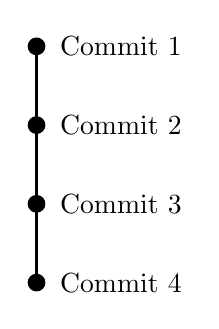
\begin{tikzpicture}
                % Draw the vertical line
                \draw[thick] (0, 0) -- (0, 3);
                
                % Draw the commit nodes
                \foreach \y in {0, 1, 2, 3} {
                    \filldraw (0, \y) circle (3pt);
                }
                
                % Label the commits
                \node[right, xshift=5pt] at (0, 3) {Commit 1};
                \node[right, xshift=5pt] at (0, 2) {Commit 2};
                \node[right, xshift=5pt] at (0, 1) {Commit 3};
                \node[right, xshift=5pt] at (0, 0) {Commit 4};
            \end{tikzpicture}
            
        \end{center}
    \end{minipage}
    
\end{frame}

\begin{frame}
    \frametitle{Grenar (\emph{Branches})}

    \begin{minipage}{0.7\textwidth}

        \ti{Man kan skapa parallella utvecklingsgrenar, som sedan kan slås samman (\emph{merge}) med huvudgrenen igen.}
        
        \begin{itemize}
            \ii{Varför vill man göra det?}
            \ii{Vilka problem kan uppstå?}
        \end{itemize}
    \end{minipage}
    \hspace{.05\textwidth}
    \begin{minipage}{0.20\textwidth}
        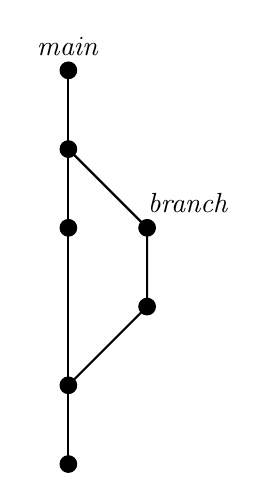
\begin{tikzpicture}
            % Rita huvudgrenen (main)
            \draw[thick] (0, 0) -- (0, 5);
            \foreach \y in {0, 1, 3, 4, 5} {
                \filldraw (0, \y) circle (3pt);
            }
            \node[above, yshift=2pt] at (0, 5) {\emph{main}};
            
            % Rita parallellgrenen (branch)
            \draw[thick] (0, 4) -- (1, 3) -- (1, 2) -- (0, 1);
            \foreach \y in {2, 3} {
                \filldraw (1, \y) circle (3pt);
            }
            \node[above, yshift=2pt, xshift=15pt] at (1, 3) {\emph{branch}};
        \end{tikzpicture}
    \end{minipage}
    
\end{frame}

\begin{frame}
    \frametitle{Varför grenar (\emph{branches})?}

    \begin{itemize}
        \ii{Grenar = parallella vägar; sidospår utan att störa huvudvägen.}
        \ii{Arbeta på olika delar av projektet samtidigt, utan att störa varandra.}
        \ii{Testa nya funktioner, experimentera säkert.}
        \ii{Skapa snabb fix för fel utan att stoppa ny utveckling.}
        \ii{Underlättar granskning och sammanslagning till huvudversion.}
        \ii{Branches i Git är lätta att skapa och använda!}
    \end{itemize}
    
\end{frame}














\begin{frame}
    \frametitle{Git-modellen}

    \begin{center}
            \includegraphics[width=\textwidth]{figs/model-rm-reset.png}
    \end{center}
    
\end{frame}


